%\documentclass[preprint,prl,superscriptaddress]{revtex4-1}
%\documentclass[twocolumn,nofootinbib]{nature}
\documentclass[onecolumn,pra,superscriptaddress,nofootinbib]{revtex4-1}

% packages
\usepackage[dvips]{graphicx} % for figures
\usepackage{amsfonts,amssymb,amscd,amsmath,amsthm}
\usepackage{enumerate}
\usepackage{epsfig}
\usepackage{subfigure}
\usepackage{xcolor}
%\usepackage[expert]{mathdesign}

\newcommand{\bra}[1]{\mbox{$\left\langle #1 \right|$}}
\newcommand{\ket}[1]{\mbox{$\left| #1 \right\rangle$}}
\newcommand{\braket}[2]{\mbox{$\left\langle #1 | #2 \right\rangle$}}

\newtheorem{theorem}{Theorem}
\newtheorem{lemma}{Lemma}
\newtheorem{corollary}{Corollary}
\newtheorem{claim}{Claim}
\newtheorem{conjecture}{Conjecture}
\newtheorem*{observation}{Observation}
\newtheorem{definition}{Definition}

\begin{document}

\title{Lecture 2: two-qubit system}

%% For REVTeX it is possible to automate superscript and e-mail callouts with the superscriptaddress option; see REVTeX4 documentation.


\author{Xiongfeng Ma}
\email{xma@tsinghua.edu.cn}
\affiliation{Center for Quantum Information, Institute for Interdisciplinary Information Sciences, Tsinghua University, Beijing 100084, China}


\begin{abstract}
In the last chapter, we have learned about one qubit system. Here, we shall learn about a two-qubit system. It turns out two-qubit system has much more fun. It will take three weeks for us to cover these materials. Guess how many qubits we can cover by the end of the course?

Two-qubit state, mixed state, Bloch ``ball", positive-operator valued measure (POVM); Super operator, purification of mixed state and POVM; Bell's inequality, CHSH/CH/Eberhard inequality; Experiment development and loopholes, entanglement; Quantum dense coding, teleportation (experiment development); Using teleportation for operation (Gottesman-Chuang'99), remote state preparation; Quantum dense coding, teleportation (experiment development); Using teleportation for operation (Gottesman-Chuang'99), remote state preparation
\end{abstract}

%\ocis{(270.5565) Quantum communications; (270.5568) Quantum cryptography.}


\maketitle %% required

\section{Review: one-qubit System}
\begin{enumerate}
\item{state: ray.}
\item{normalize state: vector.}
\item{representation way: $\ket{u}=\cos{\frac{\theta}{2}}+e^{i\theta}\sin{\frac{\theta}{2}}$. (Bloch Sphere\footnote{No standard way to visualize two or more qubits system until now.})}
\item{density matrix: $\rho = \sum_i\lambda_i\ket{\phi_i}\bra{\phi_i}$.\footnote{why we can't distinguish $\ket{u}$ and $e^{i\theta}\ket{u}$? because $\ket{u}\bra{u}=e^{i\theta}\ket{u}\bra{u}e^{-i\theta}$. Their density matrices are always the same.}}
\item{$\rho^{+} = \rho, Tr(\rho) = 1.$}
\item{$\forall \ket{\phi}, \bra{\phi}\rho\ket{\phi} \geq 0$\footnote{By physical meaning of the measurement.}.}
\item{For pure qubit, Assume $\rho = \ket{\phi}\bra{\phi}$, we have $\rho^2 = \rho.$ Also, we can get the eigenvalues and eigenvectors of $\rho$ (Assume $\ket{\Phi}$ is orthogonal of $\ket{\phi}$): 
\begin{equation}
\begin{aligned}
\rho\ket{\phi} = \ket{\phi}\braket{\phi}{\phi} = \ket{\phi}.\\
\rho\ket{\Phi} = \ket{\phi}\braket{\phi}{\Phi} = 0.
\end{aligned}
\end{equation}}

\item{$\bra{\psi}M\ket{\psi} = Tr(\bra{\psi}M\ket{\psi}) = Tr(M\ket{\psi}\bra{\psi}) = Tr(M\rho).$\footnote{$Tr(AB)=\sum_{i}\sum_j a_{ij}b_{ji} = \sum_{i}\sum_j b_{ij}a_{ji} = Tr(BA)$.}}
\end{enumerate}

\section{Notations}
Matrix tensor product $\otimes$,
%consider two matrices,
%\begin{equation} \label{2qubit:2mat}
%\begin{aligned}
%\[
%\begin{pmatrix}
%    a_{1,1} & a_{1,2} \\
%    a_{2,1} & a_{2,2}
%\end{pmatrix}
%
%\begin{pmatrix}
%    b_{1,1} & b_{1,2} \\
%    b_{2,1} & b_{2,2}
%\end{pmatrix}.
%\]
%\end{aligned}
%\end{equation}
the tensor product of two matrices is
\begin{equation} \label{2qubit:tensorproduct}
\begin{aligned}
  \begin{bmatrix}
    a_{1,1} & a_{1,2} \\
    a_{2,1} & a_{2,2} \\
  \end{bmatrix}
\otimes
  \begin{bmatrix}
    b_{1,1} & b_{1,2} \\
    b_{2,1} & b_{2,2} \\
  \end{bmatrix}
=
  \begin{bmatrix}
    a_{1,1}  \begin{bmatrix}
              b_{1,1} & b_{1,2} \\
              b_{2,1} & b_{2,2} \\
            \end{bmatrix} & a_{1,2}  \begin{bmatrix}
                                      b_{1,1} & b_{1,2} \\
                                      b_{2,1} & b_{2,2} \\
                                    \end{bmatrix} \\
     & \\
    a_{2,1}  \begin{bmatrix}
              b_{1,1} & b_{1,2} \\
              b_{2,1} & b_{2,2} \\
            \end{bmatrix} & a_{2,2}  \begin{bmatrix}
                                      b_{1,1} & b_{1,2} \\
                                      b_{2,1} & b_{2,2} \\
                                    \end{bmatrix} \\
  \end{bmatrix}
=
  \begin{bmatrix}
    a_{1,1} b_{1,1} & a_{1,1} b_{1,2} & a_{1,2} b_{1,1} & a_{1,2} b_{1,2} \\
    a_{1,1} b_{2,1} & a_{1,1} b_{2,2} & a_{1,2} b_{2,1} & a_{1,2} b_{2,2} \\
    a_{2,1} b_{1,1} & a_{2,1} b_{1,2} & a_{2,2} b_{1,1} & a_{2,2} b_{1,2} \\
    a_{2,1} b_{2,1} & a_{2,1} b_{2,2} & a_{2,2} b_{2,1} & a_{2,2} b_{2,2} \\
  \end{bmatrix}.
\end{aligned}
\end{equation}


Here, we simplify denote it as
\begin{equation} \label{2qubit:tensorsimp}
\begin{aligned}
\ket{\phi}\otimes\ket{\psi} = \ket{\phi}\ket{\psi}\\
\end{aligned}
\end{equation}


Here, we simplify denote it as
\begin{equation} \label{2qubit:tensorsimp}
\begin{aligned}
\ket{\phi}\otimes\ket{\psi} = \ket{\phi}\ket{\psi}\\
\end{aligned}
\end{equation}

\subsection{Trace}
Trace $Tr(\rho)$: summation of the diagonal terms.

Partial trace $Tr_B(\rho_{AB})$: Assume A is n-dimension state, B is m-dimension state, then $\rho_{AB}$ can be regarded as a $nm \times nm$ matrix. $Tr_B(\rho_{AB})$ is a $n\times n$ matrix, where $(Tr_B(\rho_{AB}))_{ij} = \sum_{k=1}^{m}(\rho_{AB})_{ik, jk}.$s Particularly, $Tr_B(A \otimes B) = Tr(B)A.$

\subsection{Schmidt decomposition}
For any pure state $\ket{\psi}_{AB}$ of a bipartite system, there are orthonormal bases $\{\ket{i}_A\}$ and $\{\ket{i��}_B\}$ such that:
\begin{equation} \label{Schmidt decomposition}
\begin{aligned}
\ket{\psi}_{AB}=\sum_i\sqrt{p_i}\ket{i}_A\otimes\ket{i'}_B.
\end{aligned}
\end{equation}
The subsystems $A$ and $B$ have the same eigenvalues, $p_i$s. The number of $p_i$s is called the Schmidt number of $\ket{\psi}_{AB}$. We denote that the pure state is a entangled state when the the Schmidt number is greater than one. It is easy to see that the Bell states are entangled states.




\section{Two-qubit system}

\subsection{an interesting ``paradox"}
When considering a two qubits state which is written as
\begin{equation} \label{4BellZ}
\begin{aligned}
\ket{\psi}_{AB}=\ket{0}_{A}\ket{0}_{B}+\ket{1}_{A}\ket{1}_{B}.\\
\end{aligned}
\end{equation}
When measure the system $A$ in the $Z$ basis, with probability $1/2$, the measurement result is $\ket{0}$ and the prepared state is $\ket{0}_A\ket{0}_B$. With probability $1/2$, the measurement result is $\ket{1}$ and the prepared state is $\ket{1}_A\ket{1}_B$.

That is: $$
\ket{\psi}_A = \frac{1}{\sqrt{2}}(\ket{0} + \ket{1}) = \ket{+}.
$$

Consider another two qubits state :
\begin{equation} \label{4BellZ}
\begin{aligned}
\ket{\psi}_{AB}=\ket{+}_{A}\ket{+}_{B}+\ket{-}_{A}\ket{-}_{B}.\\
\end{aligned}
\end{equation}
By similar induction way, we have
$$
\ket{\psi}_A = \frac{1}{\sqrt{2}}(\ket{+} + \ket{-}) = \ket{0}.
$$

But actually,
\begin{align}
\ket{\psi}_{AB}&=\ket{0}_{A}\ket{0}_{B}+\ket{1}_{A}\ket{1}_{B}\\
 &= 1/2(\ket{+}+\ket{-})(\ket{+}+\ket{-})+1/2(\ket{+}-\ket{-})(\ket{+}-\ket{-})\\
 &= \ket{+}_A\ket{+}_B+\ket{-}_A\ket{-}_B.
\end{align}

So now we have: $\ket{0} = \ket{+}.$ What's wrong?

\textbf{Explanation:} The key of the above paradox is that $\ket{\psi}_A$ isn't a pure state any more, we only can write it as a density matrix. The density operator of subsystem A is given by
\begin{equation} \label{4BellZ}
\begin{aligned}
\rho_A=tr_B(\ket{\psi}_{AB}\bra{\psi}_{AB})=\frac{1}{\sqrt{2}}(\ket{0}\bra{0}+\ket{1}\bra{1}).\\
\end{aligned}
\end{equation}


\subsection{EPR paradox~\cite{EPRparadox}}
Alice and Bob have a two qubits system:
$$
\ket{\psi}_{AB} = \ket{0}_{A}\ket{0}_{B}+\ket{1}_{A}\ket{1}_{B}.
$$
Alice gets qubit A, Bob gets qubit B. Then Alice goes to a planet which far from Bob. Then if Alice wants to tell 0 to B, she measures A in $\ket{+/-}$ basis; if she wants to tell 1 to B, she measures A with $\ket{0/1}$ basis.   

WOLG, We assume that after measurement for A, Alice gets $\ket{0}$. Then
for Bob, he measures B after a while with basis $\ket{0/1}$, if he gets $\ket{0}$ with probability 1, he can say Alice wants to tell him 0.

So by this process, we transform information which is faster than light. What's the problem? 

\textbf{Explanation:}For Bob, if he gets $\ket{0}$, he doesn't know which basis Alice uses. Because if Alice chooses $\ket{0/1}$ basis, Bob has $0.5$ probability to get $\ket{0}$; if Alice chooses $\ket{+/-}$ basis, Bob also has $0.5$ probability to get $\ket{0}$.

This experiments tells us, quantum has the \textbf{non-locality} and also \textbf{no-signalling} properties. 
$$
\textit{Something are changed, but we don't know.}
$$

\subsection{The properties for general density matrix}
In general, the state is represented by a density operator.
In the case where the state of the subsystem is a ray, and we say that the state is
pure. Otherwise the state is mixed. If $\rho_A=\rho_A^2$, then $\ket{\psi_A}$ is a pure state. Otherwise, the density matrix of A is
$\rho_A=\sum_a p_a\ket{a}\bra{a}$, where $\sum_ap_a=1$, $0<p_a<1$. The trace distance $tr \rho_A^2=\sum_a p_a^2<\sum_ap_a=1$.

Properties of a general density matrix
\begin{enumerate}
\item
self-adjoint: $\rho_A=\rho_A^\dag$
\item
positivity: for $\forall\ket{\psi}$, $\bra{\psi}\rho_A\ket{\psi}\ge0$
\item
completeness: $Tr(\rho_A)=1$
\end{enumerate}



\subsection{Schmidt decomposition}
For any pure state $\ket{\psi}_{AB}$ of a bipartite system, there are orthonormal bases $\{\ket{i}_A\}$ and $\{\ket{i��}_B\}$ such that:
\begin{equation} \label{Schmidt decomposition}
\begin{aligned}
\ket{\psi}_{AB}=\sum_i\sqrt{p_i}\ket{i}_A\otimes\ket{i'}_B.
\end{aligned}
\end{equation}
The subsystems $A$ and $B$ have the same eigenvalues, $p_i$s. The number of $p_i$s is called the Schmidt number of $\ket{\psi}_{AB}$. We denote that the pure state is a entangled state when the the Schmidt number is greater than one. It is easy to see that the Bell states are entangled states.


\subsection{Bell basis}
The dimension of the 2-qubit Hilbert space is 4. Thus, there are 4 basis states. Bell state basis is widely used, especially for the case involving entanglement. The 4 Bell states in the $Z$ basis are,
\begin{equation} \label{4BellZ}
\begin{aligned}
\Phi^+ &= \ket{00}+\ket{11} \\
\Phi^- &= \ket{00}-\ket{11} \\
\Psi^+ &= \ket{01}+\ket{10} \\
\Psi^- &= \ket{01}-\ket{10} \\
\end{aligned}
\end{equation}
in the $X$ basis are
\begin{equation} \label{4BellZ}
\begin{aligned}
\Phi^+ &= \ket{++}+\ket{--} \\
\Phi^- &= \ket{-+}+\ket{+-} \\
\Psi^+ &= \ket{++}-\ket{--} \\
\Psi^- &= \ket{-+}-\ket{+-} \\
\end{aligned}
\end{equation}
in the $Y$ basis are
\begin{equation} \label{4BellZ}
\begin{aligned}
\Phi^+ &= \ket{+i-i}+\ket{-i+i} \\
\Phi^- &= \ket{+i+i}+\ket{-i-i} \\
\Psi^+ &= -i(\ket{+i+i}-\ket{-i-i}) \\
\Psi^- &= i(\ket{+i-i}-\ket{-i+i}) \\
\end{aligned}
\end{equation}

Many interesting simple quantum information phenomenons come with Bell states, such as Bell's inequality, Teleportation, super dense coding, quantum key distribution, and Deutsch's algorithm.


\subsection{Bloch sphere and qubit tomography}
A useful representation of the state of a single qubit is the Bloch sphere representation. Since the overall phase is irrelevant, a pure state of a qubit can be written as
\begin{equation} \label{eq:BlochSphere}
\begin{aligned}
\ket{u} = \cos\frac{\theta}{2}\ket{0}+e^{i\varphi}\sin\frac{\theta}{2}\ket{1}.
\end{aligned}
\end{equation}
Therefore, it is convenient to represent it as a vector living the surface of a unit sphere with the spherical coordinate $(r=1,\theta,\varphi)$.

\begin{figure}[tbh]
\centering \resizebox{4cm}{!}{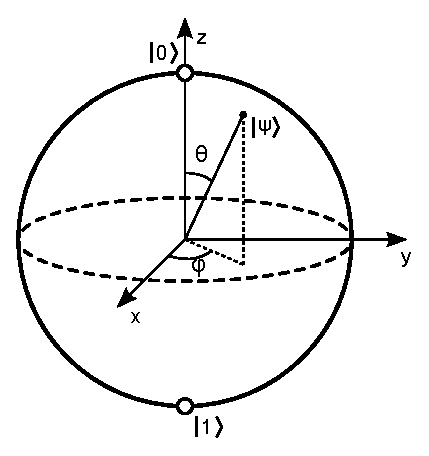
\includegraphics{epsBlochSphere.eps}}
\caption{Bloch sphere.} \label{fig:BlochSphere}
\end{figure}

In general, a qubit might be in a mixed state, and then it will be within the Bloch sphere instead on the surface. In general, the density matrix of a qubit can be written as
\begin{equation} \label{eq:rhoBloch}
\begin{aligned}
\rho &= \frac12(\sigma_0+\vec{P}\cdot \vec{\sigma}) \\
&= \frac12
    \begin{pmatrix}
      1+P_z&P_x-iP_y\\
      P_x+iP_y&1-P_z
    \end{pmatrix}
\end{aligned}
\end{equation}
where $\vec{P}=(P_x,P_y,P_z)$ is a vector and $|\vec{P}|\le1$. When $|\vec{P}|=1$, Eq.~\eqref{eq:rhoBloch} represents a pure qubit.

Quantum state tomography is the process of reconstructing the quantum state for a quantum system by proper measurements. The quantum state can be pure (vector) or in general mixed (density matrix). A set of measurements is called tomographically complete if it can uniquely identify the state. That is, the measurement outcomes are able to provide all the information about the state. In the classical physics, it corresponds to system calibration.

Let us take qubit tomography for example. As given in Eq.~\eqref{eq:rhoBloch}, the $Z$ basis measure provides the information on $P_z$. By changing the $Z$ and $X$ basis, by the Hadamard transformation, we can conclude that the $X$ basis measure provides the information on $P_x$. Similarly, the $Y$ basis measure provides the information on $P_y$. Thus, $X$, $Y$, and $Z$ measurements is tomographically complete for a qubit. Another way to put this is,
\begin{equation} \label{eq:rho2tomo}
\begin{aligned}
\rho &= \frac12[tr(\rho)\sigma_0+tr(\sigma_x\rho)\sigma_x+tr(\sigma_y\rho)\sigma_y+tr(\sigma_z\rho)\sigma_z]. \\
\end{aligned}
\end{equation}
Now, let us move a bit further, tomography for $n$ qubits,
\begin{equation} \label{eq:rhontomo}
\begin{aligned}
\rho &= 2^{-n}\sum_{v_1,v_2,\dots,v_n\in\{0,x,y,z\}}tr(\sigma_{v1}\otimes\sigma_{v2}\otimes\cdots\otimes\sigma_{vn}\rho) \sigma_{v1}\otimes\sigma_{v2}\otimes\cdots\otimes\sigma_{vn},
\end{aligned}
\end{equation}
where the sum is over all possible the identity and Pauli matrices.

In another related concept, quantum process tomography, known quantum states are used to probe a quantum process to find out how the process can be described. Similarly, quantum measurement tomography works to find out what measurement is being performed.

The general principle behind quantum state tomography is that by repeatedly performing many different measurements on quantum systems described by identical density matrices, frequency counts can be used to infer probabilities, and these probabilities are combined with Born's rule to determine a density matrix which fits the best with the observations.

\section{Positive Operator-Valued Measure}
For the bipartite state $\ket{\psi}_{AB}$ given in Eq.~\eqref{2qubit:2qubiteg}, if we only measure system $A$, the observable can be expressed as
\begin{equation} \label{2qubit:jointmeasure}
\begin{aligned}
M_A\otimes I_B
\end{aligned}
\end{equation}
where $M_A$ is a self-adjoint operator acting on system $A$. Then the expectation value of the measurement outcome is,
\begin{equation} \label{2qubit:jointmeasureExp}
\begin{aligned}
\bra{\psi}M_A\otimes I_B\ket{\psi} &= (a^* \bra{0}_{A}\bra{0}_{B}+b^*\bra{1}_{A}\bra{1}_{B}) (M_A\otimes I_B) (a \ket{0}_{A}\ket{0}_{B}+b\ket{1}_{A}\ket{1}_{B}) \\
&= |a|^2 \bra{0}M_{A}\ket{0}+|b|^2\bra{1}M_{A}\ket{1}. \\
\end{aligned}
\end{equation}
Since we know that the density matrix of $\rho_A=|a|^2\ket{0}\bra{0}+|b|^2\ket{1}\bra{1}$, Eq.~\eqref{2qubit:jointmeasureExp} can be written as,
\begin{equation} \label{2qubit:jointmeasureExprho}
\begin{aligned}
\langle M_A \rangle = tr(M_A\rho_A)
\end{aligned}
\end{equation}

We can understands the difference between the Positive Operator-Valued Measure (POVM) and PVM with the same sense that a density matrix is to a pure state.  The POVM can be used to describe the effect of PVM acts on a large system.
The operators $\{E_a\}$ form a complete set of Hermitian nonnegative operators and satisfy that:
\begin{enumerate}
\item Hermiticity: $E_a=E_a^\dag$.
\item Positivity :$\bra{\psi}E_A\ket{\psi}\ge0$.
\item Completeness: $\sum_aE_a=I$.
\end{enumerate}


\section{quantum channel}
The quantum channel is also called ``super operator". The super means that the map takes operators to operators, rather than vectors to vectors. Unitary evolution on $\mathcal{H}_A\otimes\mathcal{H}_B $ will not in general appear to be unitary if we restrict our attention to $\mathcal{H}_A$ alone. Rather, evolution in HA will be described by a quantum channel, (which can be inverted by another channel only if unitary). A general channel $\mathcal{E}$ has an operator-sum representation:
\begin{equation} \label{eq:channel}
\begin{aligned}
\mathcal{E}(\rho)=\sum_aM_a\rho M_a^\dag,\\
\sum_aM_a^\dag\rho M_a=I.\\
\end{aligned}
\end{equation}


\section{Ensembles}
A mixed state of a system A can be prepared as an ensemble of pure states in
many different ways, all of which are experimentally indistinguishable if
we observe system A alone.
\begin{equation} \label{eq:Ensembles}
\begin{aligned}
\rho_A=\sum_ip_i\ket{\psi_i}\bra{\psi_i},\sum p_i=1.
\end{aligned}
\end{equation}

For any such $\rho_A$,  we can construct a ��purification�� of $\rho_A$, $\ket{\Psi_1}_{AB}$,
\begin{equation} \label{eq:purification}
\begin{aligned}
\ket{\Psi_1}_{AB}=\sum_i \sqrt{p_i}\ket{\psi_i}_A\ket{\alpha_i}_B,
\end{aligned}
\end{equation}
where $\{\ket{\alpha_i}_B\}$ are mutually orthogonal and normalized.
The relation between two purifications, $\ket{\Psi_1}_{AB}$ and $\ket{\Psi_2}_{AB}$ , is given by,
\begin{equation} \label{eq:purifications}
\begin{aligned}
\ket{\Psi_1}_{AB}=(I_A\otimes U_B)\ket{\Psi_2}_{AB},
\end{aligned}
\end{equation}
the two states differ by an unitary change of basis acting in $\mathcal{H}_B$ alone.


\section{Quantum Teleportation}
The seminal work by C.~H.~Bennett, G.~Brassard, C.~Cr\'epeau, R.~Jozsa, A.~Peres and W.~K.~Wootters is published in 1993 \cite{PhysRevLett.70.1895}. Quantum teleportation is a process by which quantum information can be transmitted (exactly, in principle) from one location to another, with the help of classical communication and previously shared quantum entanglement between the sending and receiving location. Because it depends on classical communication, which can proceed no faster than the speed of light, it cannot be used for superluminal transport or communication of classical bits. It also cannot be used to make copies of a system, as this violates the no-cloning theorem.

\begin{figure}[hbt]
\centering \resizebox{6cm}{!}{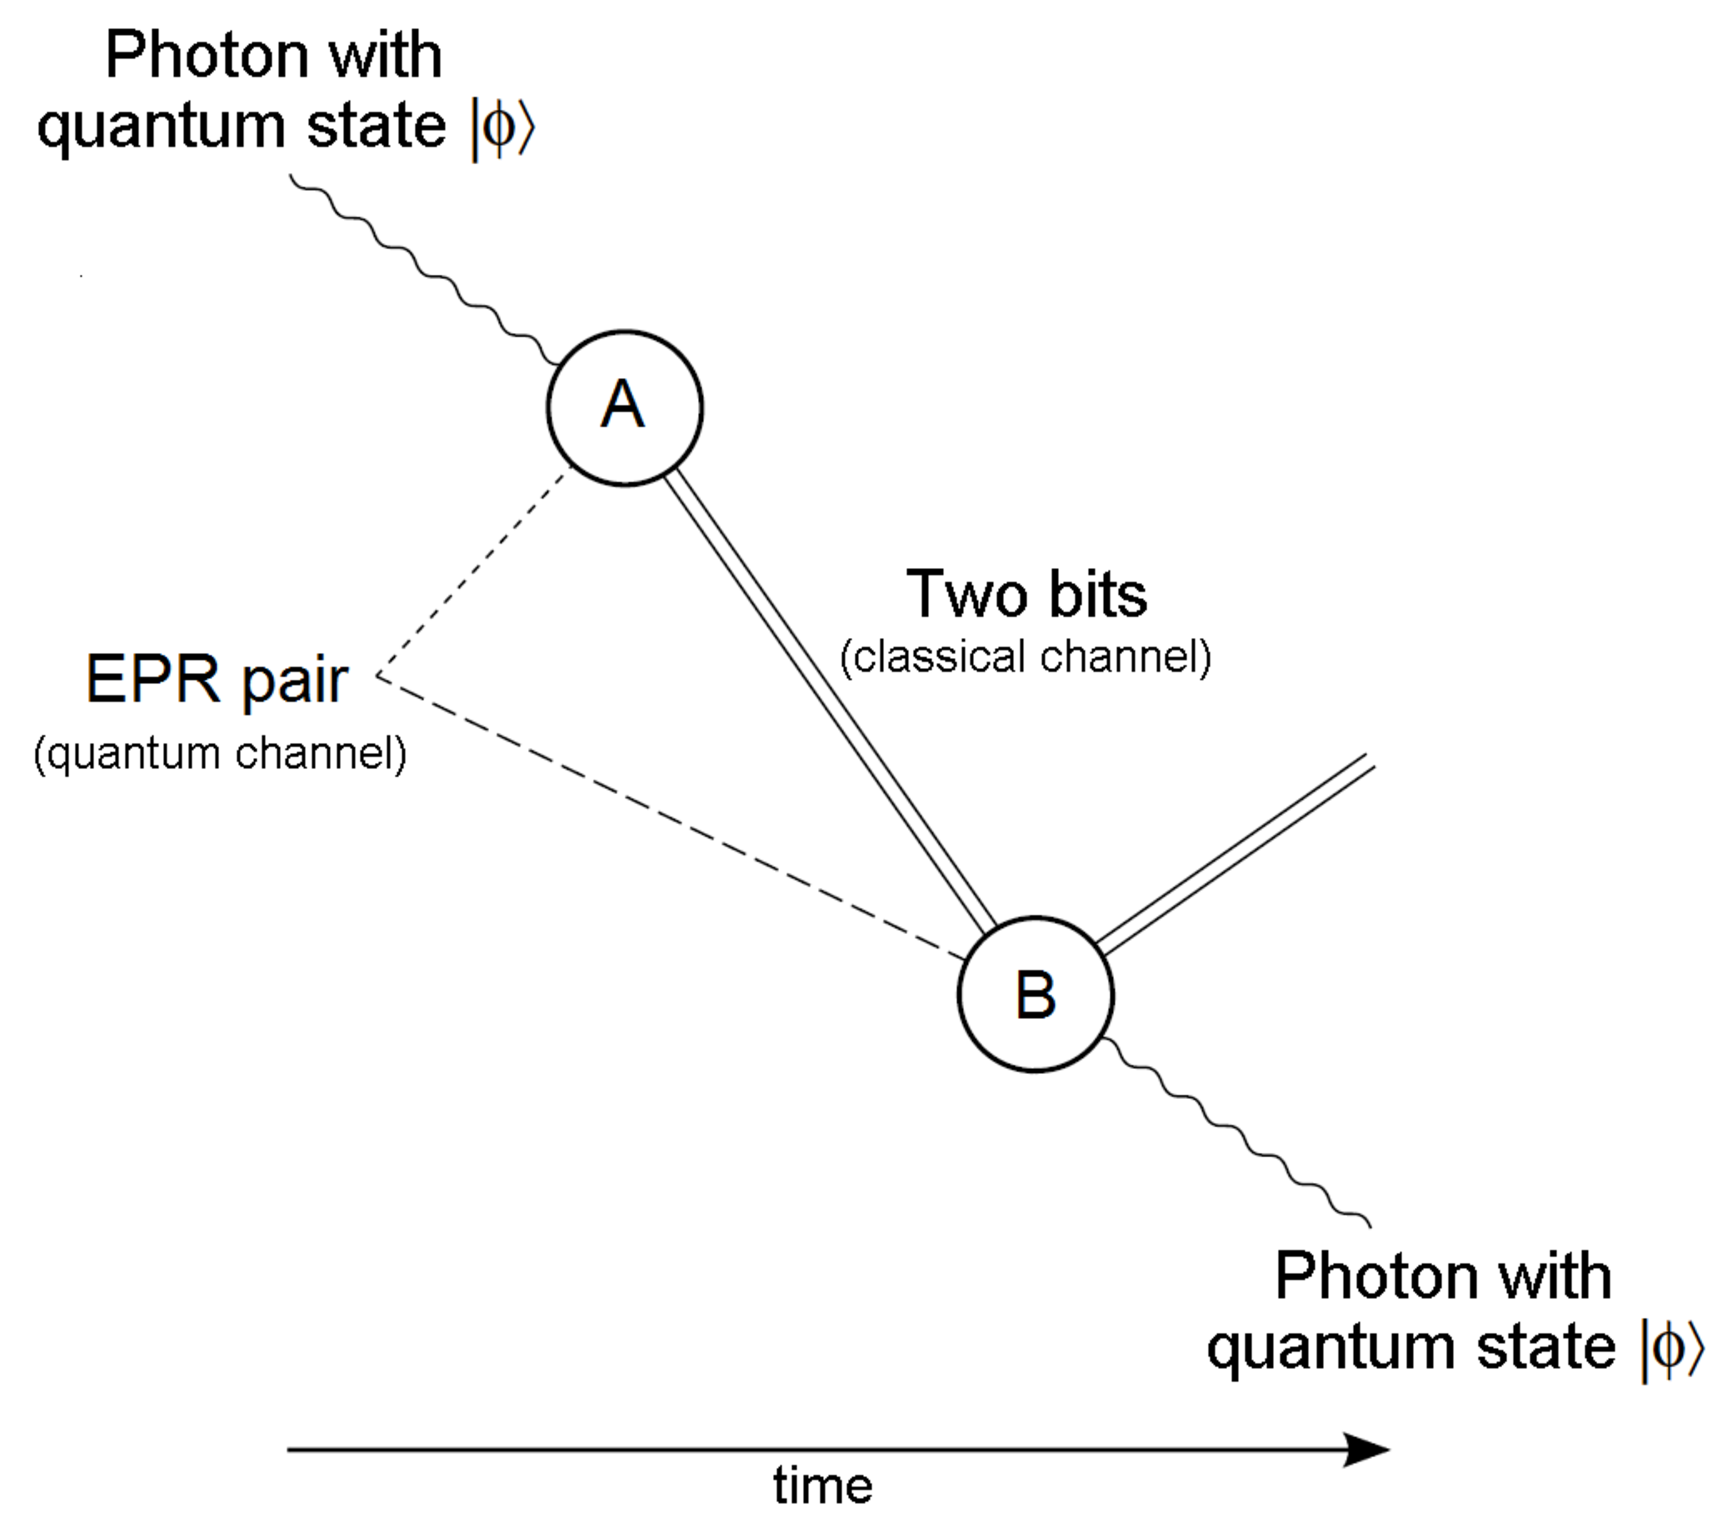
\includegraphics{epsTeleportation.eps}}
\caption{Schematic diagram for quantum teleportation.} \label{Fig:Teleport}
\end{figure}

Quantum teleportation can be regarded as a secure way to transfer information \cite{Lo1999Science}.


%%%%%%%%%%%%%%%%%%%%%%%%%%%%%%%%%%%%%%%%
% choose a style
%\bibliographystyle{ieeetr}
%\bibliographystyle{unsrt}
\bibliographystyle{apsrev4-1}
%%%%%%%%%%%%%%%%%%%%%%%%%%%%%%%%%%%%%%%%


%%%%%%%%%%%%%%%%%%%%%%%%%%%%%%%%%%%%%%%%
% choose a .bib file
%\bibliography{Ch2TwoQubit4_1_}
%%%%%%%%%%%%%%%%%%%%%%%%%%%%%%%%%%%%%%%%
\end{document}

